\chapter{什么是智能}
\label{chap:definition}

\section{如何定义智能}

人类心智和认知分为神经、心理、语言、思维、文化五个层级。在人类认知的所有五个层级上,人工智能都是在模仿人类智能; 人工智能是在不断进步的,但在总体上并未超过人类智能。在语言、思维和文化层级上,即在高阶认知层级上,目前人工智能都远逊于人类智能。事实上,人工智能和人类智能这两种智能方式是截然不同的。机器学习也只是对人类认知能力的一种模仿,不能作过高的评价,不必惊慌,更不能人为地制造恐慌。著名的塞尔人工智能理论“中文房间论证”的模型和标准并未过时, 根据这个论证, 数字计算机(digital computer) 永远不会具有人类智能,因此,在可预见的未来也不会出现超过人类智能的人工智能\cite{renjidazhan}。

智力或智能是指生物一般性的精神能力。这个能力包括以下几点:推理、理解、计划、解决问题、抽象思维、表达意念以及语言和学习的能力。
	
智能化一般指使原本没有智能的机械、设备、生产方式等主题拥有部分智能。这种智能属于“人工智能”。

按照弱人工智能(Artificial Narrow Intelligence)和强人工智能(Artificial General Intelligence)的划分,目前的人工智能通通属于弱人工智能,即让机器具有某种智能的行为(can machine act intelligently)。尽管在某些特殊的领域,专家系统已经达到甚至超过人类智能,例如 19 年前战胜卡斯帕罗夫的“深蓝”和刚刚战胜李世石的 AlphaGo,也包括在当代工业生产线上广泛使用的各种专业机器人。但这些人工智能包括“深蓝”和 AlphaGo 的人工智能都只是属于弱人工智能。而强人工智能, 即让机器能够真正地像人类一样地思考(can machine really think) ,目前只是出现在好莱坞的科幻电影里或强人工智能者的信仰里。迄今为止,并没有任何一部真正理解人类语言的机器,因此更不会有像人一样能够进行创造性思维的机器和具有人一样的文化生存方式的机器\cite{renjidazhan}。

因此尽管“智能”这个词很“火热”,但是其在某些领域的应用目前还处于很初级的阶段,对于液压系统来说,一般性的机电液一体化研究也能被扣上“智能”的帽子。我们看待“智能液压”问题,一定不能站在极高的角度来苛求液压系统的“智能”。

\section{液压系统和智能}

液压与气压传动系统主要由以下五部分组成\cite{yeyakeben}:能源装置、执行元件、控制元件、辅助元件、工作介质。

% \begin{multicols}{5}
% \begin{itemize}
% 	\item 能源装置
% 	\item 执行元件
% 	\item 控制元件
% 	\item 辅助元件
% 	\item 工作介质
% \end{itemize}
% \end{multicols}

机器的组成,有以下部分\cite{jixieshejikeben}:原动机部分、传动部分、执行部分、检测和控制部分、辅助部分。

% \begin{multicols}{5}
% \begin{itemize}
% 	\item 原动机部分
% 	\item 传动部分
% 	\item 执行部分
% 	\item 检测和控制部分
% 	\item 辅助部分
% \end{itemize}
% \end{multicols}

\begin{figure}[!htp]
	\centering
	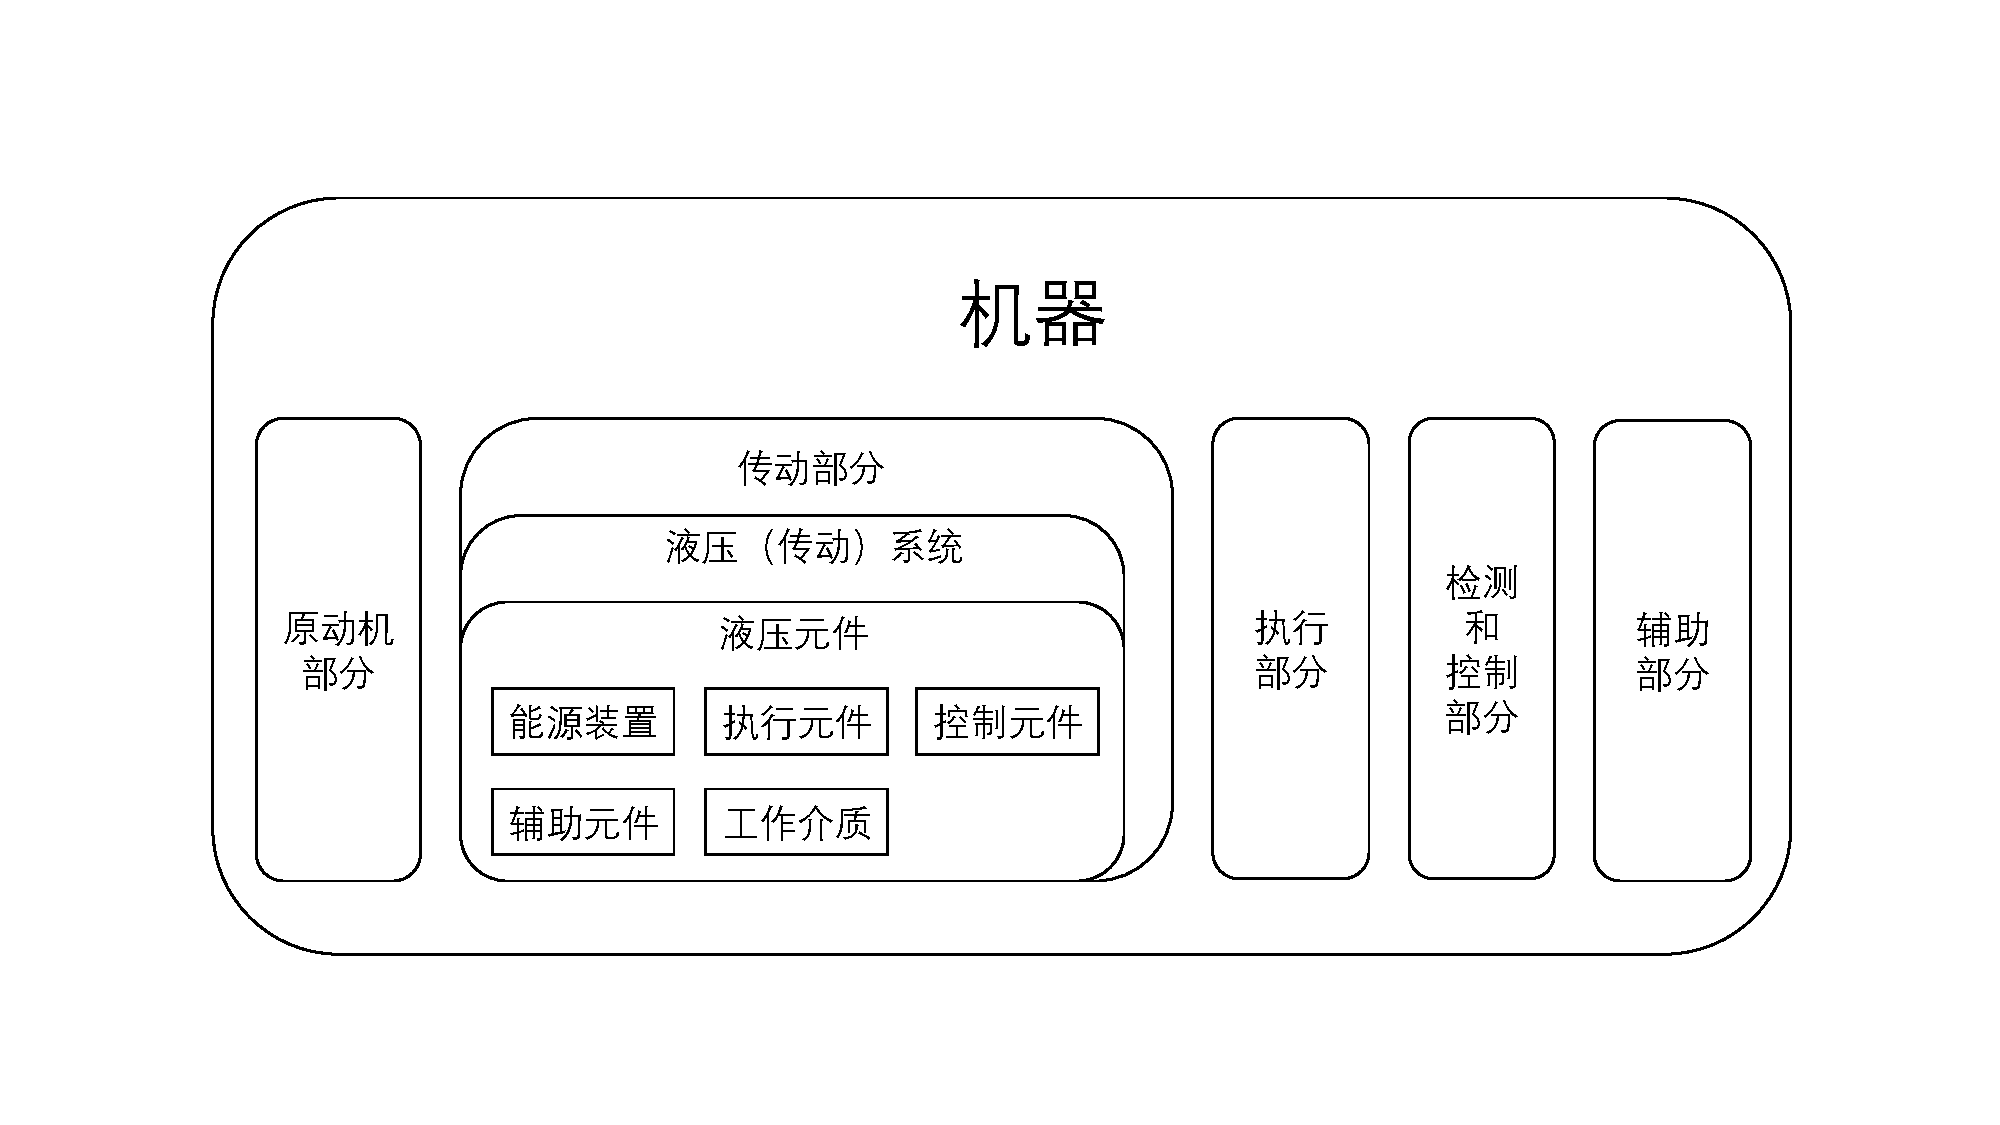
\includegraphics[width=\textwidth]{IMG/jiqizucheng.pdf}
	\bicaption[机器组成图]
		{机器组成图}
		{machine composition diagram}
	\label{fig:jiqizucheng}
\end{figure}

如图\ref{fig:jiqizucheng}所示,一台机器可以分层次得拆分为不同的子系统。

显然,液压传动系统只是一个机器的一个部分,液压传动系统和机器各自的组成部分名字虽然有所相似,但是实际上意义不同。

只要机器的某个部分被“智能化”了,那么其父概念就可以被认为被“智能化”。比如只要液压传动系统中的某个执行元件是智能元件,那么这个液压系统就是智能系统,这个机器就是智能机器。
